\chapter{Geometry}

\section{Basics}

A determinant of a $2x2$ matrix is defined as
\[
    \left\vert
        \begin{array}{cc}
            a & b \\
            c & d \\
        \end{array}
    \right\vert
    = a d - b c
\]

\section{java.awt.geom}

The \texttt{java.awt.geom} and \texttt{java.awt} packages have, albeit limited, facilities
for geometric problems.  There are classes to represent shapes - see 
\href{http://docs.oracle.com/javase/6/docs/api/java/awt/Shape.html}{java.awt.Shape}, including
lines, ellipses, rectangles and some curves.

\begin{itemize}
\item "is contained in".  java.awt.geom.Shape provide a contains() method to test if a point
    is contained in a shape.  Contains() returns true if the point is in the interior, and false
    if the point is outside the shape. However, it may return true or false if the point is 
    on the shape boundary.

\item "intersects."  Tests if a shape intersects with a rectangle.
    Can also test if two lines or line segments intersect, but cannot find the point of
    intersection.

\end{itemize}

\section{Coordinate Geometry}

\subsection{Line/Line Intersection}
\index{Line/Line Intersections}

\begin{figure}
    \centering
    % Wikipedia Public Domain image
    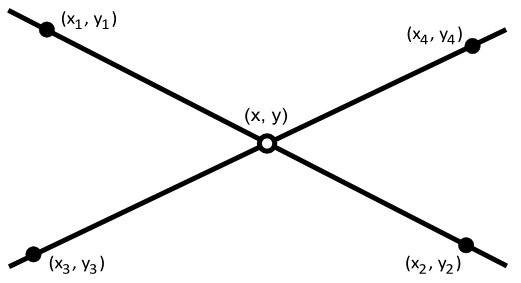
\includegraphics[height=1.5in]{Line-Line_Intersection.png}
    \caption{Line line intersection}
    \label{fig:linelineintersect}
\end{figure}

\[
\begin{array}{ll}
P_x = \frac{\begin{vmatrix} 
                \begin{vmatrix} x_1 & y_1\\
                                x_2 & y_2
                \end{vmatrix} & 
                \begin{vmatrix} x_1 & 1\\
                                x_2 & 1
                \end{vmatrix} \\\\ 
                \begin{vmatrix} x_3 & y_3\\
                                x_4 & y_4
                \end{vmatrix} & 
                \begin{vmatrix} x_3 & 1\\
                                x_4 & 1
                \end{vmatrix} 
            \end{vmatrix} }{
            \begin{vmatrix} 
                \begin{vmatrix} x_1 & 1\\
                               x_2 & 1
                \end{vmatrix} &  
                \begin{vmatrix} y_1 & 1\\
                                y_2 & 1
             \end{vmatrix} \\\\ 
             \begin{vmatrix} x_3 & 1\\
                             x_4 & 1
             \end{vmatrix} & 
             \begin{vmatrix} y_3 & 1\\
                             y_4 & 1 
             \end{vmatrix} 
            \end{vmatrix}}

&

P_y = \frac{\begin{vmatrix} 
                \begin{vmatrix} x_1 & y_1\\
                                x_2 & y_2
                \end{vmatrix} &  
                \begin{vmatrix} y_1 & 1
                              \\y_2 & 1
                \end{vmatrix} \\\\ 
                \begin{vmatrix} x_3 & y_3\\
                                x_4 & y_4
                \end{vmatrix} & 
                \begin{vmatrix} y_3 & 1\\
                                y_4 & 1
                \end{vmatrix} 
            \end{vmatrix} }
           {\begin{vmatrix} 
               \begin{vmatrix} x_1 & 1\\
                               x_2 & 1
               \end{vmatrix} &
               \begin{vmatrix} y_1 & 1\\
                               y_2 & 1
            \end{vmatrix} \\\\ 
            \begin{vmatrix} x_3 & 1\\
                            x_4 & 1
            \end{vmatrix} & 
            \begin{vmatrix} y_3 & 1\\
                            y_4 & 1
            \end{vmatrix} 
     \end{vmatrix}}\,\!
\\

\end{array}
\]

The determinants can be written out as:
\begin{align*}
    (P_x, P_y)= \bigg(&\frac{(x_1 y_2-y_1 x_2)(x_3-x_4)-(x_1-x_2)(x_3 y_4-y_3 x_4)}{(x_1-x_2)(y_3-y_4)-(y_1-y_2)(x_3-x_4)}, \\
                      &\frac{(x_1 y_2-y_1 x_2)(y_3-y_4)-(y_1-y_2)(x_3 y_4-y_3 x_4)}{(x_1-x_2)(y_3-y_4)-(y_1-y_2)(x_3-x_4)}\bigg)
\end{align*}

Source: \href{http://en.wikipedia.org/wiki/Line-line_intersection}{http://en.wikipedia.org/wiki/Line-line\_intersection}.

\paragraph{Notes}
\begin{itemize}
\item Parallel or coincident lines:
    Denominator will be zero:
    \[
        (x_1 - x_2) (y_3 - y_4) - (y_1 - y_2) (x_3 - x_4) = 0
    \]
\item One line horizontal ($y_1 = y_2$ or $y_3 = y_4$), the other vertical ($x_1 = x_2$ or $x_3 = x_4$) will also
    give a 0 determinant, but the lines will intersect.  Handle as special case if problem allows it.

\item Intersection point may be outside the given segments.

\item If you only need to know if two lines intersect, but not where, use java.awt.geom.Line2D.intersects.
\end{itemize}

\paragraph{Code}

\inputminted{java}{code/lineintersection.java}

%
%
%

\subsection{Area of a Polygon}
\index{Polygon!Area}
\index{Area!Polygon}
\index{Polygon}

The signed area of a planar non-self-intersecting polygon with vertices $(x_1, y_1), \dots, (x_n, y_n)$ is
\[
    A = \frac{1}{2} \left(
        \left\vert
        \begin{array}{cc}
            x_1 & x_2 \\
            y_1 & y_2 \\
        \end{array}
        \right\vert
        +
        \left\vert
        \begin{array}{cc}
            x_2 & x_3 \\
            y_2 & y_3 \\
        \end{array}
        \right\vert
        + \ldots +
        \left\vert
        \begin{array}{cc}
            x_n & x_1 \\
            y_n & y_1 \\
        \end{array}
        \right\vert
        \right)
\]

Figure~\ref{fig:polygonareadeterminant} shows how to multiply this out
\[
    A = \frac{1}{2} \left(
        x_1 y_2 - x_2 y_1
      + x_2 y_3 - x_3 y_2
      + \ldots +
      + x_{n-1} y_n - x_n y_{n-1}
      + x_{n} y_1 - x_1 y_n
      \right)
\]

(Source: Mathworld~\cite{mathworldpolygonarea})

\begin{figure}
    \centering
    % Wikipedia Public Domain image
    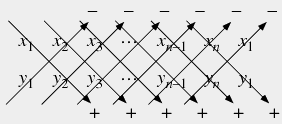
\includegraphics[height=1.5in]{PolygonArea_1000.png}
    \caption{Line line intersection}
    \label{fig:polygonareadeterminant}
\end{figure}

\paragraph{Notes}
\begin{itemize}
\item Works for any simple polygon (concave or convex)
\item Does not work for complex polygons (when any edges intersect)
\item A is positive if points are in counterclockwise order, negative if points are in clockwise order.
    See the use Math.abs() in code below.
\item Triangle and any Quadrilateral are, of course, just special cases.
\end{itemize}

\paragraph{Code}
\inputminted{java}{code/polygonarea.java}

